%%%%% Physik Kompendikum -- Wellen und Optik %%%%%
%% 03 Wellen %%


%Some sample text to be displayed above the first subsection

%\subsection{Prinzip}

%Ein Zyklotron besteht aus Zwei hohlen, halbzylindrischen und Duanden an denen eine Spannung mit unterschiedlichem Vorzeichen anliegt, und darüber bzw. darunter liegende Magneten, die ein homogenes Magnetfeld erzeugen. Zudem gibt es einen Einlass und einen Auslass für Teilchen.

%\begin{wrapfigure}{r}{0.4\textwidth} \label{Zyklo}
%
%	\vspace{-10pt}
%	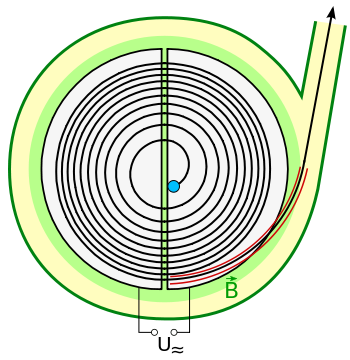
\includegraphics[width=0.35\textwidth]{Zyklotron_Prinzipskizze02.png}
%	\vspace{-13pt}
%	\caption{Prinzipskizze eines Zyklotrons}
%	\vspace{-5pt}	
%	
%\end{wrapfigure}

%\subsubsection{Anwendung}

% Some Formula:

%\begin{equation}
%	x= \frac{y \cdot 13 \pi z}
%			{\cos \alpha}
%\end{equation}

%%%%%%%%%%%%%%%%%%%%%%%
% Eigentlicher Beginn %
%%%%%%%%%%%%%%%%%%%%%%%

\subsection{Diagramme von Wellen} \label{subsec:diagramm_welle}

Einer Welle reicht ein Diagramm zur Darstellung nicht aus. Da es sehr viele Oszillatoren gibt, die alle zu unterschiedlichen Zeiten zu schwingen beginnen, bräuchte man ein Elongation-Zeit-Diagramm (\referenz{subsec:diagramm_schwingung}) für jedes Teilchen, oder ein 3-dimensionales Diagramm.

Allerdings reichen zwei Diagramme, davon ein Elongation-Zeit-Diagramm eines beliebigen Teilchens und ein Elongation-Strecke-Diagramm (auch bekannt als \glqq Standbild\grqq) zu einem beliebigen Zeitpunkt, um alle Kenngrößen der Welle erfassen zu können.



\subsection{Kenngrößen}


\subsubsection[Amplitude]{Amplitude: $y_{max}$ o. $s_{max}$ o. $\hat{y}$ o. $\hat{s}$ (Basiseinheit: $m$)}

\textbf{Kategorie: Schwingung \textit{eines} Oszillators}

Die maximale Elongation (=\glqq Auslenkung\grqq) der Schwingungen der einzelnen Oszillatoren.



\subsubsection[Periodendauer]{Periodendauer: $T$ (Basiseinheit: $s$)}

\textbf{Kategorie: Schwingung \textit{eines} Oszillators}
	
Die Zeit, die es dauert bis einer der schwindenden Körper an der selben Stelle von der selben Richtung aus angelangt ist. Beispielsweise vom positiven Schwingungsmaximum (\glqq Berg\grqq) zum nächsten oder von der Nullstelle (\glqq Ruhelage\grqq) zur 2. darauffolgenden Nullstelle.

Davon abgeleitet:
\begin{itemize}
	\item Frequenz: $f=\frac{1}{T}$ (Basiseinheit: $Hz=\frac{1}{s}$)
	
	Anzahl der Perioden pro Sekunde.
	\item Winkelgeschwindigkeit: $\omega=2 \pi f=\frac{2 \pi}{T}$ (Basiseinheit: $\frac{rad}{s}$)
		
	Änderung des Winkels über der Zeit, wobei eine ganze Periode mit $360 \degree$ im Grad oder, im Physikunterricht verwendet, mit $2 \pi$ im Bogenmaß (eng: \glqq Radian\grqq) bezeichnet wird.\footnote{Umrechnung des Winkels $\alpha$ von Grad nach Bogenmaß: $\alpha_{rad} = \alpha_{deg} \cdot \frac{2\pi}{360 \degree} = \alpha_{deg} \cdot \frac{\pi}{180 \degree} $}
\end{itemize}



\subsubsection[Wellenlänge]{Wellenlänge: $\lambda$ (Basiseinheit: $m$)}

\textbf{Kategorie: Oszillatorsystem}

Der räumliche Abstand zwischen 2 Wellenbergen im Elongation-Strecke-Diagramm, der Abstand eines Nulldurchlaufs mit dem zweiten darauffolgenden.



\subsubsection[Ausbreitungsgeschwindigkeit]{Ausbreitungsgeschwindigkeit: $c$ (Basiseinheit: $\frac{m}{s}$)}

Die Ausbreitungsgeschwindigkeit ist eigentlich keine echte Kenngröße, da sie nicht in der Wellengleichung auftaucht. Trotzdem ist sie hilfreich um $\lambda$ oder $f$ zu berechnen. Die Gleichung lautet:

\begin{equation} \label{eq:wellen_c}
	c=\lambda \cdot f=\frac{\lambda}{T}
\end{equation}



\subsection{Wellengleichungen}

Die Wellengleichung gibt die Elongation des Teilchens mit dem Abstand $x$ zum Ausgangspunkt zum Zeitpunkt $t$ an:

\begin{equation} \label{eq:wellengleichung_y}
	y(x,t) = y_{max} \cdot sin{ (2\pi(\frac{t}{T}-\frac{x}{\lambda})) }
\end{equation}

Zur Herleitung aus der Schwingungsgleichung muss Folgendes beachtet werden. Die Zeit $t_x$ bis das räumliche Teilchen $x$ von der Front der Welle erfasst wird, lässt sich recht einfach berechnen. Gebraucht wird dabei die Ausbreitungsgeschwindigkeit $c=\frac{\lambda}{T}$ die generelle Formulierung der Geschwindigkeit $v=\frac{s}{t}$:

\begin{align*}
	t   &= \frac{s}{v} \\
	t_x &= \frac{x}{c} \\
	t_x &= \frac{x \cdot T}{\lambda}
\end{align*}

Analog zur Verschiebung nach rechts von beispielsweise einer Parabel, muss der Term für $t_x$ von $t$ in der Schwingungsgleichung abgezogen werden. Damit ist die Variable $x$ mit in der Gleichung und der Term \glqq kompensiert\grqq{} den \glqq Offset\grqq{}, der sich durch das spätere Erfassen ergibt:

\begin{align*}
	y(x,t) &= y_{max} \cdot sin{[\omega \cdot (t-\frac{x}{\lambda} \cdot T)]} \\
	y(x,t) &= y_{max} \cdot sin{[\frac{2\pi}{T} \cdot (t-\frac{x}{\lambda} \cdot T)]} \\
	y(x,t) &= y_{max} \cdot sin{[2\pi \cdot (\frac{t}{T}-\frac{x}{\lambda \cdot T} \cdot T)]} \\
	y(x,t) &= y_{max} \cdot sin{[2\pi \cdot (\frac{t}{T}-\frac{x}{\lambda})]}
\end{align*}



\subsection{Weitere Gleichungen und Gesetze}

\subsubsection{Wellenfront}

\paragraph{Erreichen eines beliebigen Teilchens}

Analog zu $v=\frac{s}{t}$:

\begin{equation*}
	t=\frac{x}{\lambda}
\end{equation*}












